\chapter{Paramor}\label{chapter:paramor}
In this chapter, I will describe Paramor, the system I have selected to build upon in this thesis. Paramor was introduced by Christian Monson in his PhD thesis \citep{monson09}. Its goal is unsupervised discovery of inflectional paradigms and using them for morpheme segmentation. 

To model partial paradigms, Monson uses \emph{schemes}. A scheme is defined by a set of candidate suffixes (c-suffixes, see Section \ref{sec:paramor_init}). The set of candidate stems (c-stems) adherent to a scheme is obtained deterministically by selecting all c-stems which can form a word (present in the corpus) with each of the scheme's c-suffixes. This is the main difference between schemes and Goldsmith's signatures, where each stem can be assigned only to a single signature.

Definition of schemes implies that with adding more c-suffixes into a scheme, number of c-stems can only drop or stay the same. Schemes form a lattice when we consider partial ordering defined by c-suffix set inclusion. Figure \ref{fig:scheme_lattice}, taken from \citep{monson09}, illustrates a part of a scheme lattice for an English corpus. The highlighted scheme, (\e{0, ed, ing, s}) has 106 adherent c-stems. Adding the c-suffix \e{ly} causes a drop to only 4 c-stems, while removing the c-suffix \e{s} increases the c-stem count to 201.

\begin{figure}[p]
\centering
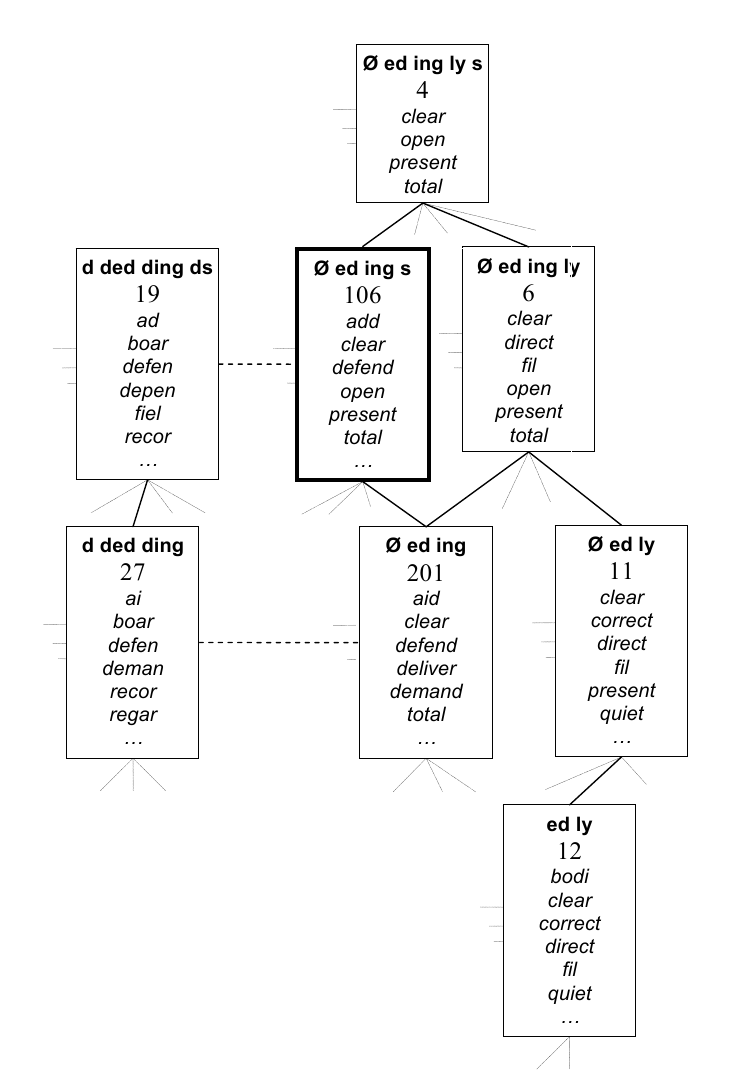
\includegraphics[scale=0.6]{schemeLattice.png}
\caption{Example part of a scheme lattice. Source: \citep{monson09}}
\label{fig:scheme_lattice}
\end{figure}

\section{Steps in Paramor's pipeline}

\subsection{Initialisation}\label{sec:paramor_init}
In the first step, sets of candidate stems (c-stems) and candidate suffixes (c-suffixes) are populated by considering every possible split into stem and suffix for every word in the corpus.

\subsection{Bottom-up Search}

Next phase of the algorithm performs a bottom-up search in the scheme lattice, starting with schemes containing exactly one c-suffix. For each of them, Paramor ascends the lattice, adding one c-suffix at a time until a stopping criterion is met. C-suffix selected for adding is the one with the biggest c-stem ratio. C-stem ratio is the ratio between the number of c-stems in the candidate higher-level scheme and the current scheme. When the highest possible c-stem ratio falls under 0.25, search stops. 

For illustration, let's use the lattice from Figure \ref{fig:scheme_lattice} and assume that the search has reached the (\e{0, ed, ing}) scheme, which has 201 adherent c-stems. There are two schemes the search can continue to: (\e{0, ed, ing, ly}) with 6 c-stems and (\e{0, ed, ing, s}) with 106 c-stems. The algorithm selects the scheme with the highest number of c-stems -- (\e{0, ed, ing, s}) and checks whether the c-stem ratio is above 0.25. The ratio is 106 / 201 = 0.53 and the search moves to the highlighted scheme. Then there is only one possibility to continue: (\e{0, ed, ing, s, ly}) with only 4 c-stems, which is rejected due to the c-stem ratio 4 / 106 = 0.04.

\subsection{Scheme Clustering}

Resulting schemes are then subjected to agglomerative bottom-up clustering. To determine proximity of two clusters, sets of (word) types generated by the clusters are measured by cosine similarity.\footnote{proximity($X$,$Y$) = $\frac{|X \cap Y|}{\sqrt{|X||Y|}}$} Cluster generates a set of types which is union of sets generated by the schemes it contains. In order to be merged, clusters must satisfy some conditions, e.g. for any two suffixes in the cluster, there must be a stem in the cluster which can combine with both of them.

\subsection{Pruning}

After clustering phase, there are still too many clusters remaining and pruning is necessary. In the first pruning step, clusters which generate only small number of types are discarded. Then Paramor tries to identify clusters modelling incorrect morpheme boundary in a Harrisian fashion by using letter entropy.

\subsection{Segmentation}

Remaining clusters can be used to segment the `training' corpus or a previously unseen text. For every word in the text, every possible division between stem $t$ and suffix $f$ is examined. If there is a cluster containing $f$ and another suffix $f'$ such that $t.f'$ is a word from the training corpus or the text, Paramor declares morpheme boundary between $t$ and $f$. In this way, more than one morpheme boundary may be found in single word. For example, the algorithm analyses \e{talks} as \e{talk} + \e{s} using the scheme cluster (0, \e{s}, \e{ing}) if \e{talk} or \e{talking} is found in the corpus. 

\section{Results and discussion}

Paramor took part in Morpho Challenge 2008\footnote{\url{http://research.ics.tkk.fi/events/morphochallenge2008/}} with excellent results, especially when combined with Morfessor. Both algorithms achieved precision higher than recall, so a natural idea was to design a combined analyser, returning the union of Paramor's and Morfessor's hypothesised morpheme boundaries. The combined analyser outperformed the other competitors in all 5 of the test languages.\footnote{In Competition 1, which directly evaluated placing of the morpheme boundaries. In Competition 2, which applied the analyses in an IR system, Paramor+Morfessor won in 1 of the 3 languages.} 

Useful feature of Paramor is that besides being able to segment texts, it outputs the scheme clusters in a human-readable way. Examining the clusters may help getting basic insight into grammatical structure of an unknown language.

A certain disadvantage of Paramor is that it does not handle the phonological/gra\-phe\-mic changes triggered by the affixation, such as the ones shown in Table \ref{table:matka}. Thus, it faces a similar problem as the engineering approach to morphology (see Section \ref{sec:engineer}) -- the need to create much larger number of paradigms. Unlike in the engineering approach, where paradigms are entered manually, Paramor  must find the evidence for the paradigms in the corpus. The richer the inflection of the language is, the more problematic sparsity becomes. An attempt to improve the algorithm by working with allomorphic variants of stems is presented in the following chapter.
